The CMS detector was designed with two primary physics goals in mind.
First, to study the properties of the Higgs boson; in particular, the nature of electroweak symmetry breaking for which the Higgs mechanism is responsible\footnote{Note that during the design of the CMS detector, the Higgs boson was theorized to exist but had not yet been discovered.}.
Second, to reveal signs of physics beyond the Standard Model which might be present at the TeV scale.
This section discusses technical design aspects of the CMS detector and how they support the physics goals of the CMS experiment.
\subsection{General Design Concepts} \label{sec:cms_overview}
The CMS detector is over 20m in length and nearly 15m in diameter -- it is ``compact'' only in the context of the tremendous size of a detector needed to facilitate the physics goals for which it was designed.
The various components of the CMS detector are shown in Fig.~\ref{fig:cms_schematic}, with humans shown to illustrate the scale (banana not available).

\begin{figure} [htbp!]
    \centering
    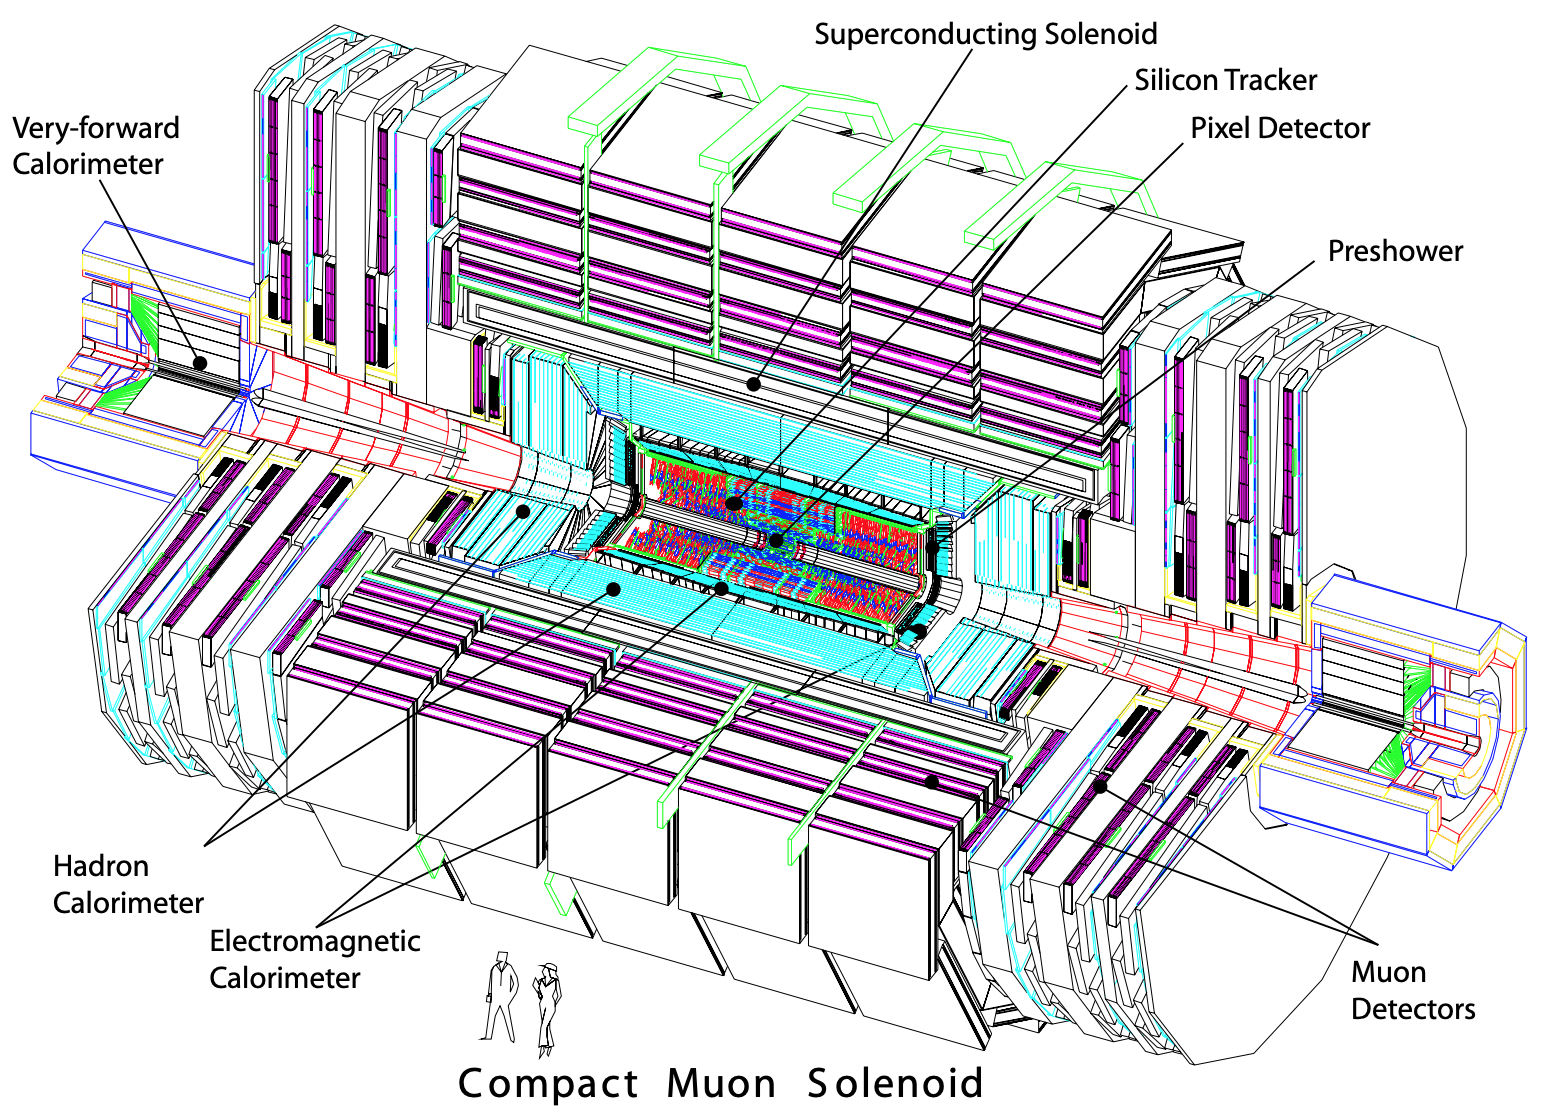
\includegraphics[width=0.8\linewidth]{figures/cms/cms_detector_schematic.png}
    \caption{Schematic of the various components of the CMS detector. Taken from~\cite{Chatrchyan:2008aa}.}
    \label{fig:cms_schematic}
\end{figure}

As its name suggests, the primary feature of the CMS detector is a superconducting solenoid providing a magnetic field of 4~T.
The purpose of the magnetic field is to bend the path of charged particles originating from inelastic proton-proton interactions: the precise spatial resolution of the tracker and muon system allows one to determine a particle's radius of curvature, in turn allowing one to determine the particle's momentum.
Excellent momentum resolution of charged particles supports nearly every physics analysis performed with the CMS detector, but is especially important for determining the invariant mass of heavy resonances (e.g. studying the properties of the Higgs boson in the H $\to$ ZZ$^{*} \to 4l$ channel), distinguishing between hadronic jets which originate from b quarks from those which originate from gluons or light-flavor quarks (e.g. the H $\to$ bb decay channel and searches for new physics involving final states with b-jets), and for precise resolution of the missing transverse energy (e.g. final states with neutrinos or searches for new physics involving final states with undetected dark matter or supersymmetry candidate particles).

The other major components of the detector include: 
\begin{itemize}
    \item The tracker, which allows for identification and measurement of the momenta of charged particles.
    \item The electromagnetic calorimeter (ECAL), which allows for identification and momenta measurement of electrons and photons, particularly important for H $\to \gamma \gamma$ physics.
    \item The hadronic calorimeter (HCAL), which assists in the identification and momentum resolution of charged hadrons and provides the only handle on measuring neutral hadrons.
    \item The muon system, which enables better momentum resolution of very high energy ($\mathcal O$(TeV)) muons (while the tracker excels in providing good momentum resolution for lower energy, $\mathcal O$(GeV) muons).
\end{itemize}
Each of these components is described in greater detail in the following subsections.

A design consideration common to multiple subdetector components is the goal of hermeticity: a fully hermetic detector is able to measure particles emerging in any direction from an inelatic collision.
In other words, a hermetic detector has full coverage of the $4\pi$ steradians of solid angle surrounding the interaction point.
The CMS detector is not fully hermetic, as it is practically impossible to measure particles which emerge parallel to the LHC's proton beams.
Still, the CMS detector is able to measure very forward particles (with ``forward'' meaning ``close to parallel with the beam axis''), aiding the nearly complete reconstruction of the final state of a given pp interaction, which is essential for resolution of the missing transverse energy.

To expand upon the concepts of hermeticity and the identification of forward particles, we must first introduce the coordinate system used to describe the CMS detector.
Given the cylindrical shape of the detector, standard cylincdrical coordinates form the basis of the coordinate system: the $\hat{z}$-axis is defined as the axis along which the proton beams travel, and the $\hat{\phi}$ direction then coincides with the detector's circular symmetry perpendicular to the beam axis.
Instead of the typical polar angle $\hat{\theta}$, position is usually expressed in terms of pseudorapidity, defined in terms of $\theta$ as
\begin{equation}
    \eta = -\ln \Bigg[ \tan \bigg(\frac{\theta}{2}\bigg) \Bigg].
\end{equation}
A pseudorapidity of $\eta = 0$ corresponds to a direction perpendicular to the beam axis, while $\eta = \infty$ corresponds to a direction parallel to the beam axis.
Pseudorapidity is convenient for a number of reasons, including the fact that it is nearly Lorentz invariant under boosts along the $\hat{z}$-axis.
We say that it is ``nearly'' Lorentz invariant as this is only true for massless particles.
However, at the LHC, the transverse momentum of a given particle is typically sufficiently larger than the mass ($\pT >> m$) such that the pseudorapidity is approximately Lorentz invariant. 

Much of the reason for CMS's 20m of length in the direction of the beam axis is motivated by the goal of hermeticity.
The forward calorimeter (described in greater detail in Sec.~\ref{sec:cms_hcal}) provides coverage up to pseudorapidities of $|\eta| \leq 5.0$.
Pairing the extensive range in pseudorapidities with the CMS detector's complete coverage in the $\hat{\phi}$-direction, the CMS detector is nearly hermetic, aiding the resolution of missing transverse energy and consequently the ability to infer the presence of undetected particles.
The exact coverage of each of the detector subcomponents is discussed in greater detail in the following subsections.

\subsection{Solenoid}
The solenoid installed in the CMS detector is over 12~m in length and 6m in diameter, capable of providing a 4~T magnetic field.
The purpose of such a strong magnetic field is to bend the trajectories of charged particles (as illustrated in Fig.~\ref{fig:cms_transverse_view}, allowing CMS to measure their momentum, mass, and charge.
Fig.~\ref{fig:cms_transverse_view} depicts the three major classes of particles which have their trajectories curved by the magnetic field produced by the solenoid: an electron (red), a charged hadron (green), and a muon (blue).
Measurements of the momenta of electrons are also aided by the ECAL (described in Sec.~\ref{sec:cms_ecal}), those of charged hadrons are also aided by the HCAL (described in Sec.~\ref{sec:cms_hcal}), and those of muons are also aided by the muon system (described in Sec.~\ref{sec:cms_muon_system}).

\begin{figure} [htbp!]
    \centering
    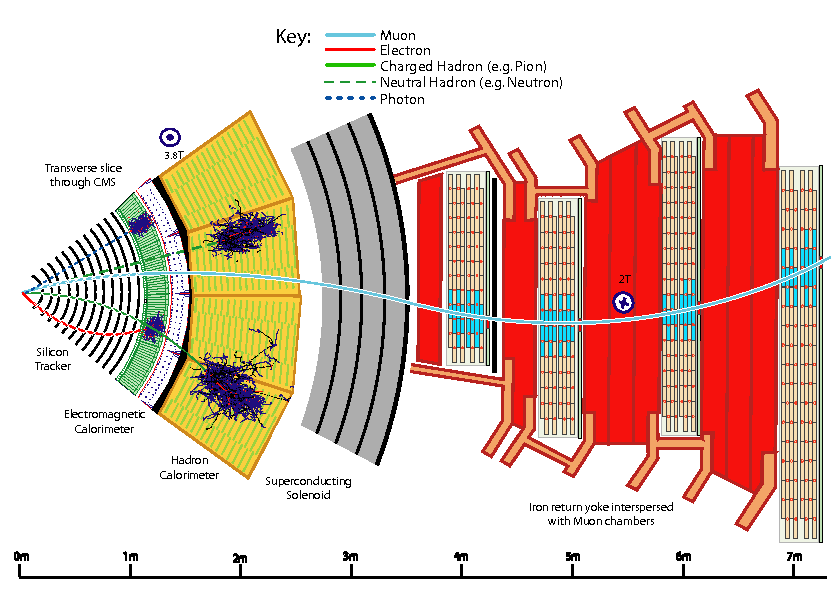
\includegraphics[width=\linewidth]{figures/cms/cms_transverse_view.png}
    \caption{Depiction of a transverse slice of the CMS detector, along with trajectories of particles of different types. Taken from~\cite{Sirunyan:2270046}.}
    \label{fig:cms_transverse_view}
\end{figure}

The solenoid is installed around the the tracker (Sec.~\ref{sec:cms_tracker}), the ECAL (Sec.~\ref{sec:cms_ecal}), and the HCAL (Sec.~\ref{sec:cms_hcal}) which is why the solenoid must be so large.
In order to support the massive current (over $10^4$~A) required for the magnetic field, the solenoid is constructed with superconducting Niobium-Titanium (NbTi), and its temperature must be kept sufficiently low to ensure superconductivity of the NbTi. 

\subsection{Tracker} \label{sec:cms_tracker}
The innermost component of the CMS detector is the silicon tracker, and its primary aim is to provide the precise reconstruction of charged particles and secondary vertices (an inelastic pp collision is deemed a ``primary vertex'' while decays of particles produced from a primary vertex are deemed ``secondary vertices'').
The tracker is nearly 6~m in length and 2.5~m in diameter, composed of an inner pixel detector with three layers ranging from 4-10~cm and an outer silicon strip tracker with ten layers ranging to 1.1~m.
Both the pixel detector and the silicon strip tracker are accompanied by endcap disks on either end of the barrel, extending the pseudorapidity coverage to $|\eta| \leq 2.5$.
Between the data-taking periods corresponding to 2016 and 2017, the inner pixel detector was upgraded~\cite{Botta:2285433}, extending the coverage of the tracker up to $|\eta| \leq 3.0$.
As shown in Fig.~\ref{fig:cms_tracker_upgrade}, the number of fake tracks, the impact parameter resolution, and the vertex resolution are each improved as well, resulting in an approximately 10\% improvement in the b-tagging efficiency for a fixed fake rate.

\begin{figure} [htbp!]
    \centering
    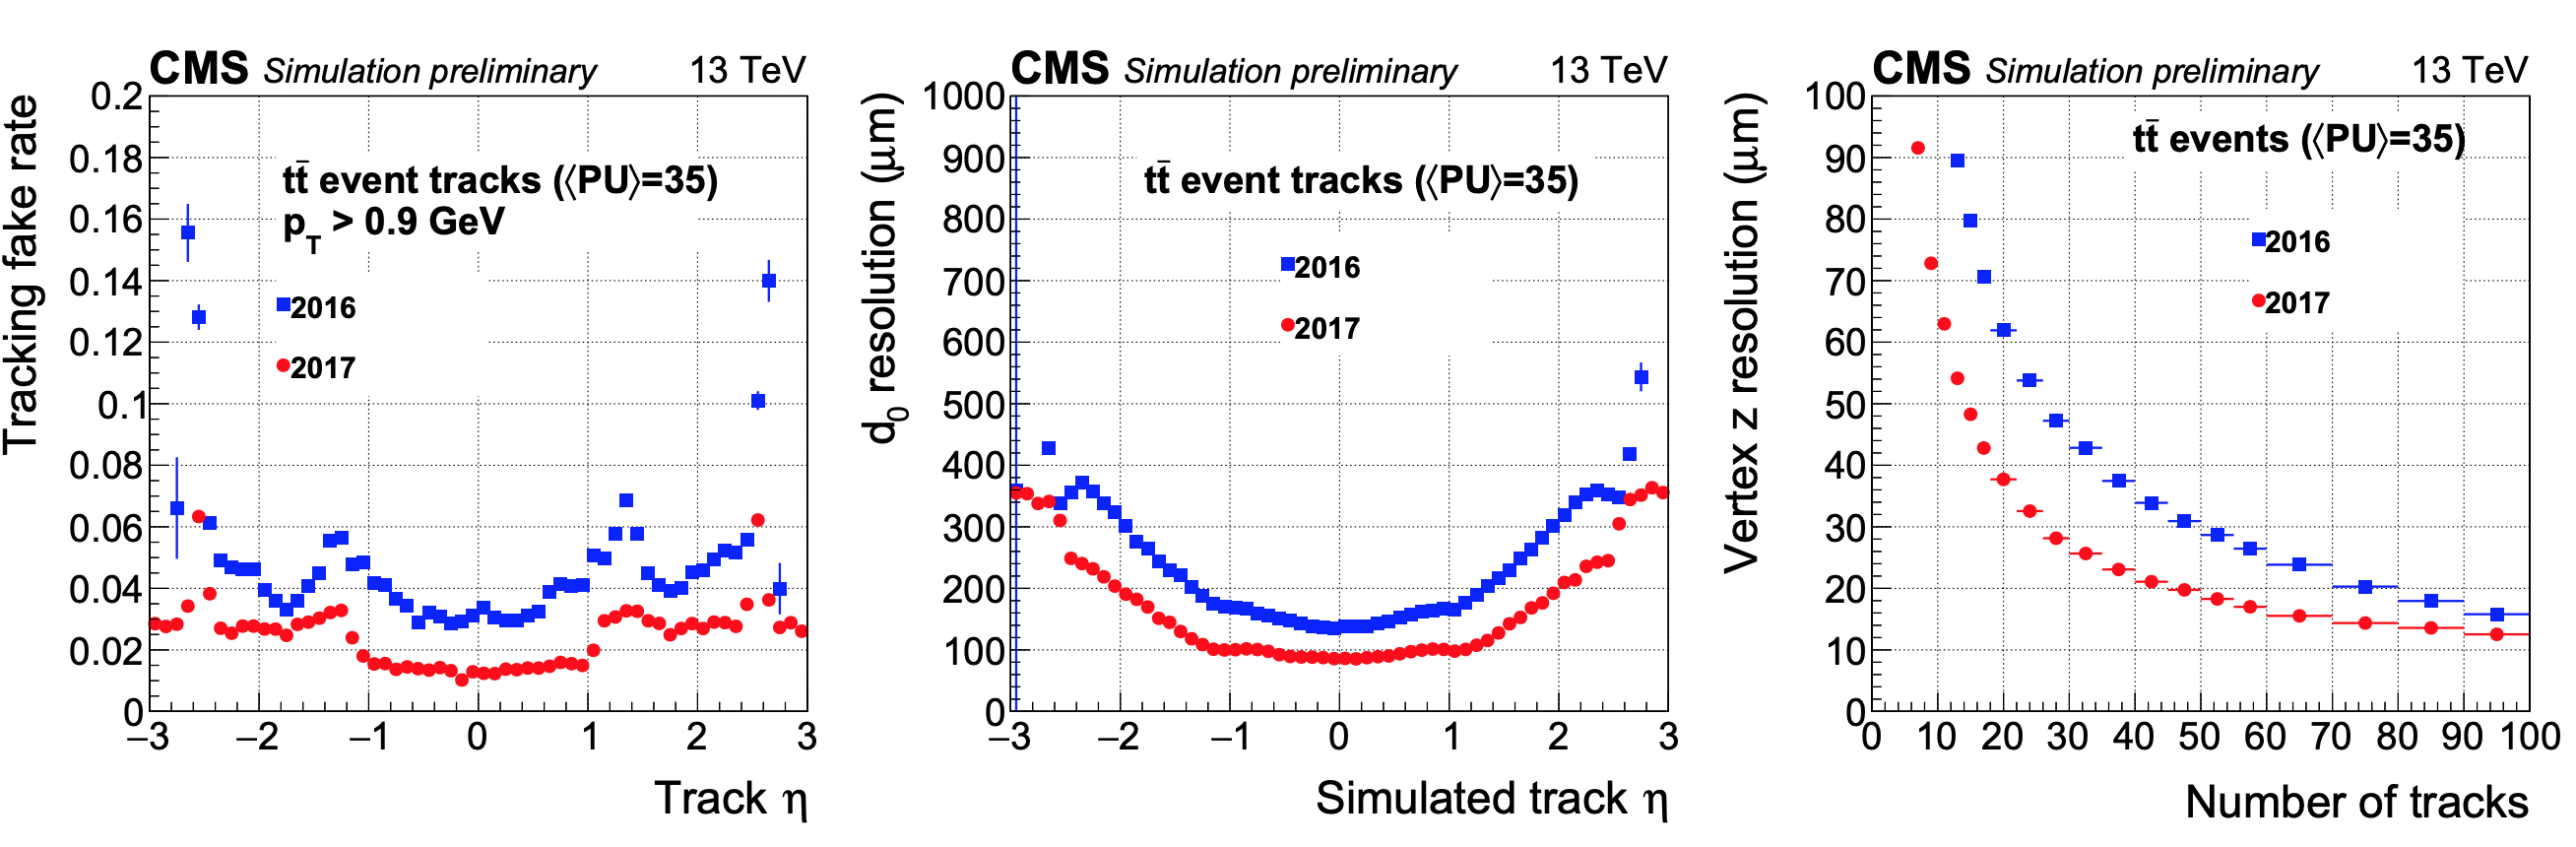
\includegraphics[width=\linewidth]{figures/cms/cms_pixel_upgrade.png}
    \caption{Comparison of tracker performance before and after the upgrade to the pixel detector, performed in between the 2016 and 2017 data-taking periods. Taken from~\cite{Botta:2285433}.}
    \label{fig:cms_tracker_upgrade}
\end{figure}

The primary design considerations for the tracker include the following:
\begin{itemize}
    \item Ability to reconstruct a large number of charged particles in each bunch crossing, with $\mathcal O(1000)$ charged particles expected from a single bunch crossing at the LHC design luminosity of $\mathcal L = 10^{34}$~cm$^{-2}$~s$^{-1}$ (corresponding to about 20 individual pp interactions).
    \item Ability to reconstruct charged particles with precise temporal resolution, with bunch crossings separated by a distance corresponding to 25~ns.
    \item Minimal interaction of photons with the tracker material, as precise measurements of photons are vital to studying Higgs physics in the \Hgg decay channel.
\end{itemize}

The first two considerations are in direct conflict with the third consideration: a tracker with high granularity and fast response implies large power density of electronics, which requires efficient cooling. This increases the material budget of the tracker, increasing the chances of bremsstrahlung and photon conversions, which in turn degrade the ECAl's photon energy resolution. 
An acceptable compromise providing both execllent tracking and excellent photon resolution was achieved with the tracker design depicted in Fig.~\ref{fig:cms_tracker_schematic}.

\begin{figure} [htbp!]
    \centering
    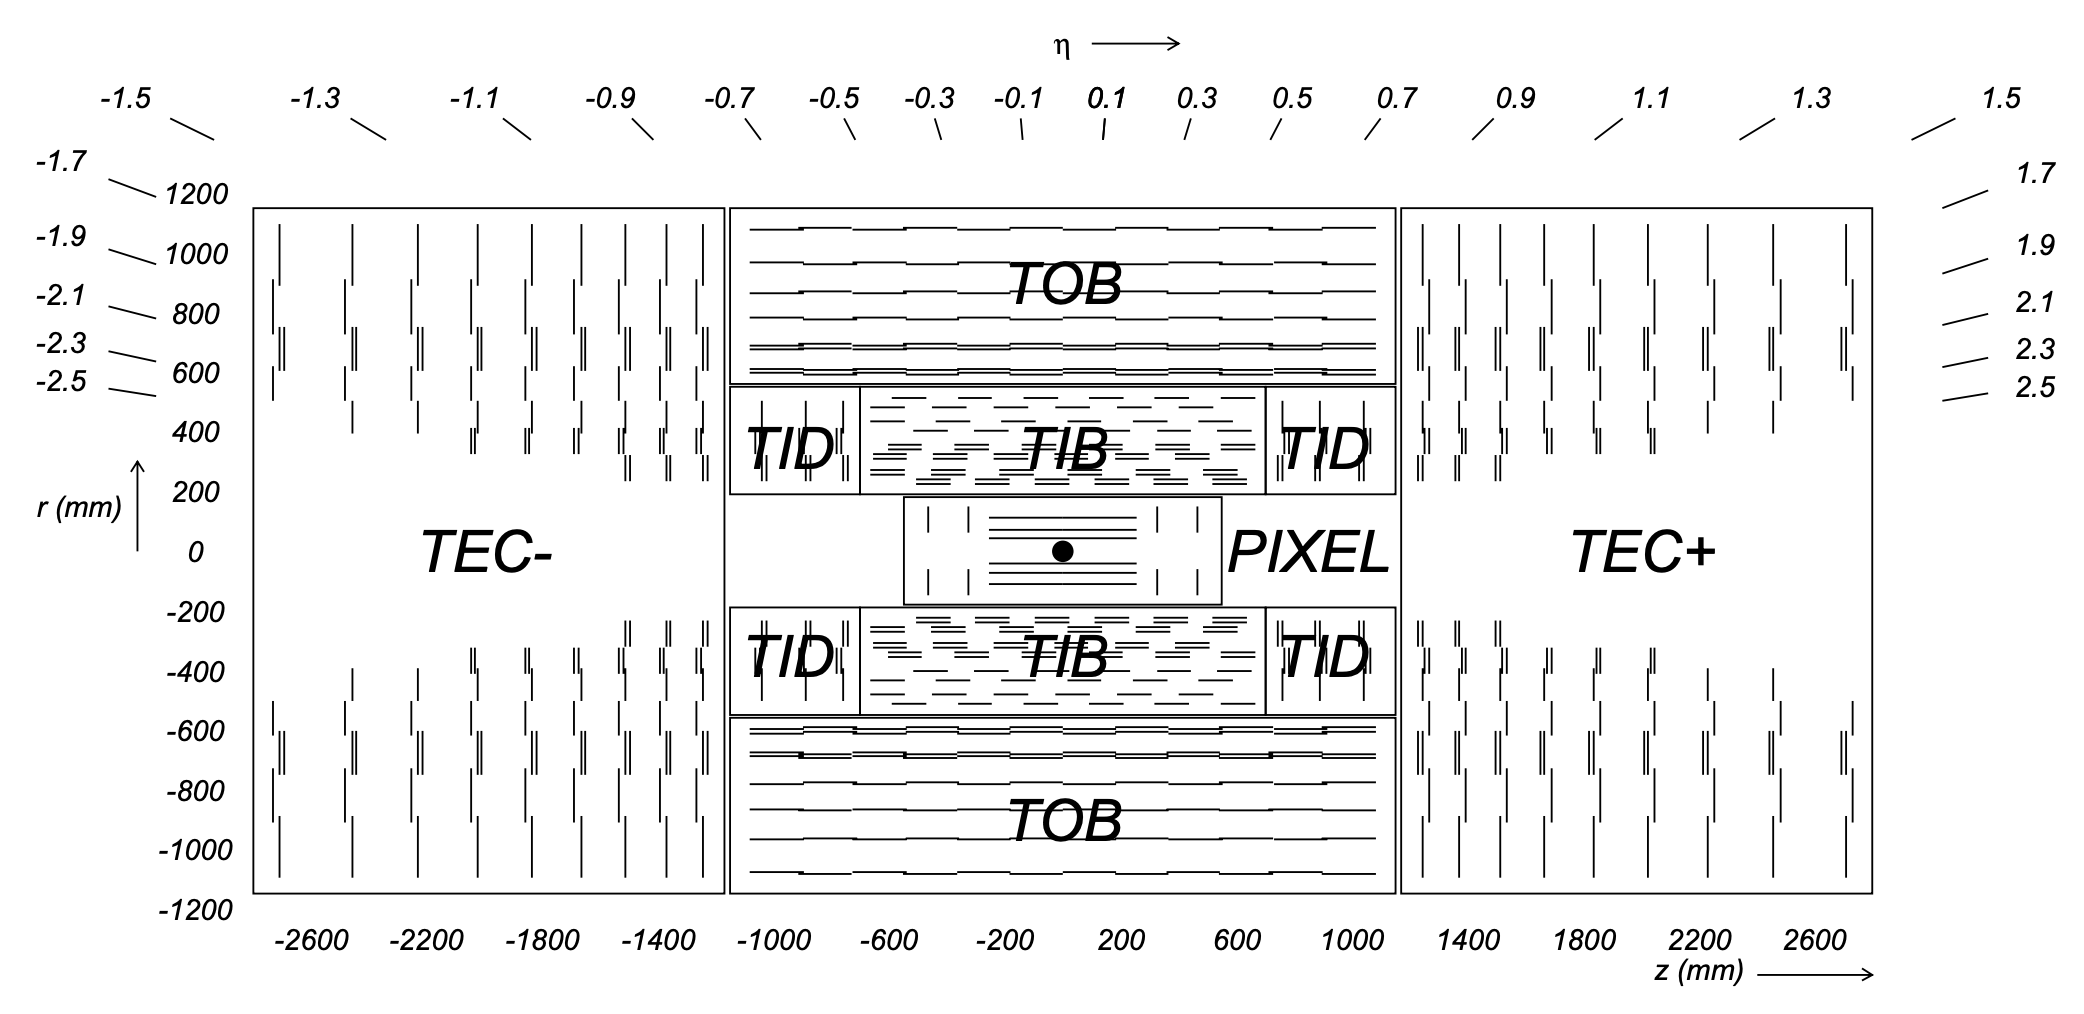
\includegraphics[width=0.8\linewidth]{figures/cms/cms_tracker_schematic.png}
    \caption{Schematic of the CMS tracker from a cross-sectional viewpoint. TIB, TOB, TID, and TEC represent the tracker inner barrel, tracker outer barrel, tracker inner disk, and tracker endcap components, respectively. Taken from~\cite{Chatrchyan:2008aa}.}
    \label{fig:cms_tracker_schematic}
\end{figure}

The material budget for the CMS tracker is shown in Fig.~\ref{fig:cms_tracker_budget}, showing the thickness of the tracker material in terms of the characteristic radiation lengths $X_0$ (for electromagnetic particles, e.g. electrons and photons) and characteristic nuclear interaction lengths $\lambda_I$ (i.e. for hadrons).
The tracker thickness in terms of both radiation lengths and nuclear interaction lengths is lowest in the most central part of the barrel and increases in the more forward components, accounting for one of the reasons that CMS achieves better energy resolution for very central particles.

\begin{figure} [htbp!]
    \centering
    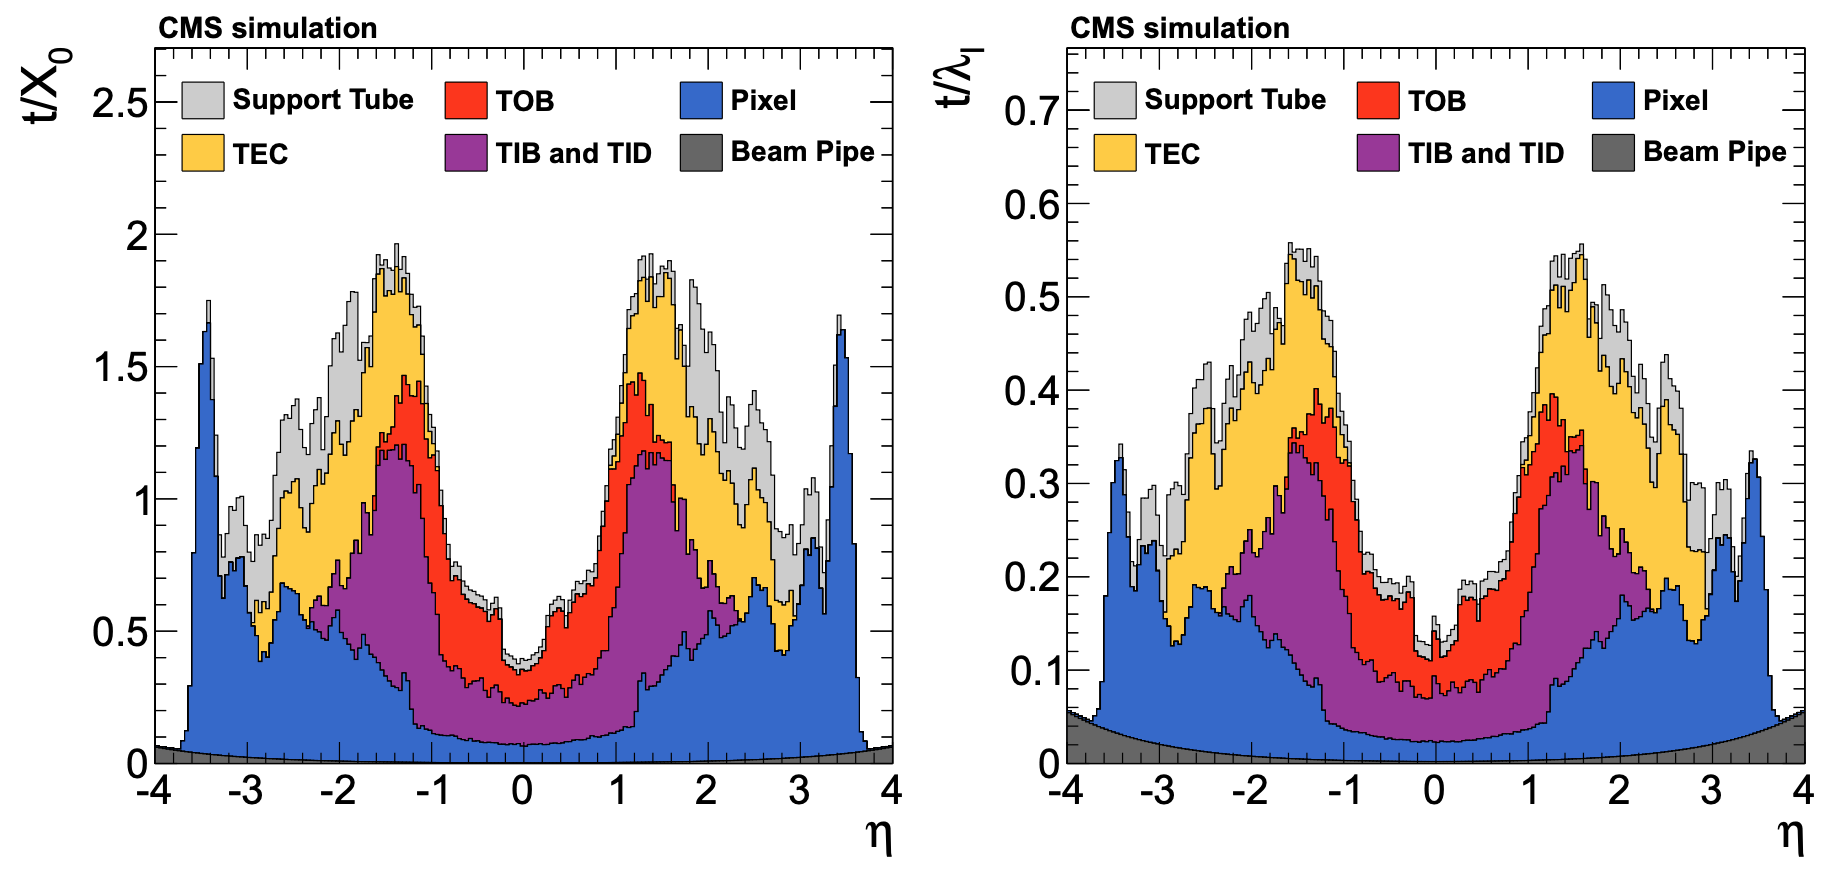
\includegraphics[width=\linewidth]{figures/cms/cms_tracker_budget.png}
    \caption{The material budget for the CMS tracker shown for both the characteristic radiation lengths of electromagnetic interactions (left) and the characteristic nuclear interaction lengths of hadronic interactions (right), with the contributions of each of the tracker subcomponents shown individually. Taken from~\cite{Chatrchyan:1704291}.}
    \label{fig:cms_tracker_budget}
\end{figure}

The tracking effieciency achieved by the CMS tracker is shown in Fig.~\ref{fig:cms_tracker_eff}, for muons, pions, and electrons as a function of their transverse momentum.
In general, the tracker achieves higher efficiency for muons than for electrons or pions, as electrons are more likely to emit radiation via bremsstrahlung and charged pions may undergo nuclear interactions with the tracker material.
Energy resolution of high \pT ($\mathcal O(TeV)$) muons is assisted by the muon system, as shown in Fig.~\ref{fig:cms_muon_vs_tracker}.

\begin{figure} [htbp!]
    \centering
    \begin{tabular}{c c c}
        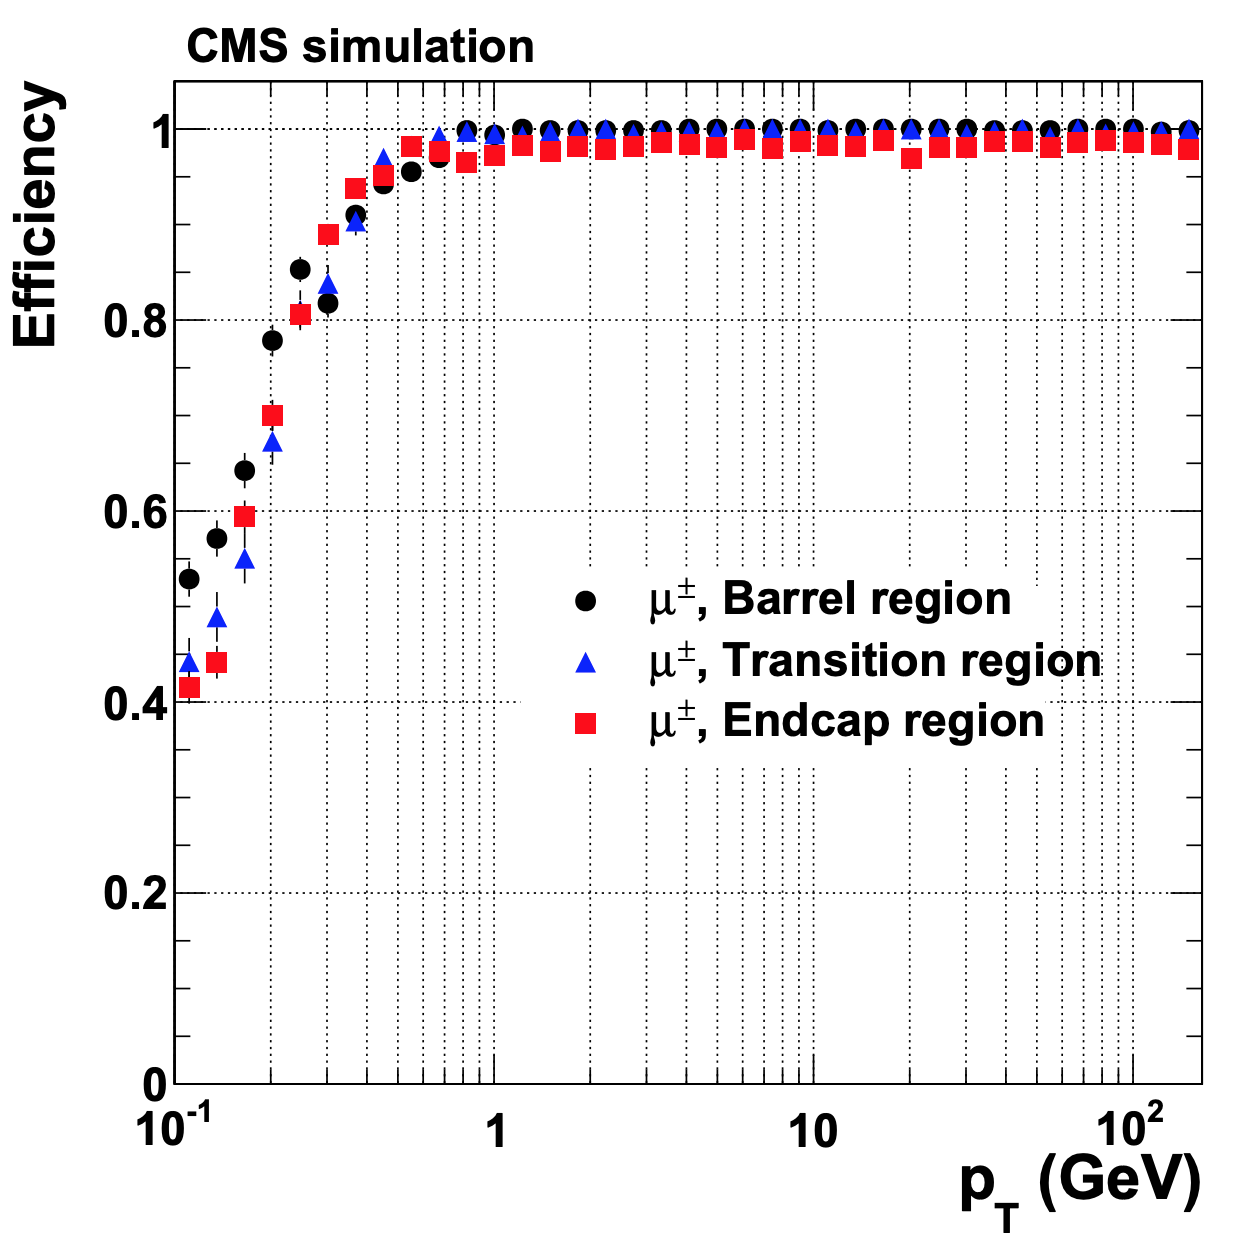
\includegraphics[width=0.31\linewidth]{figures/cms/cms_tracker_muon.png} &
        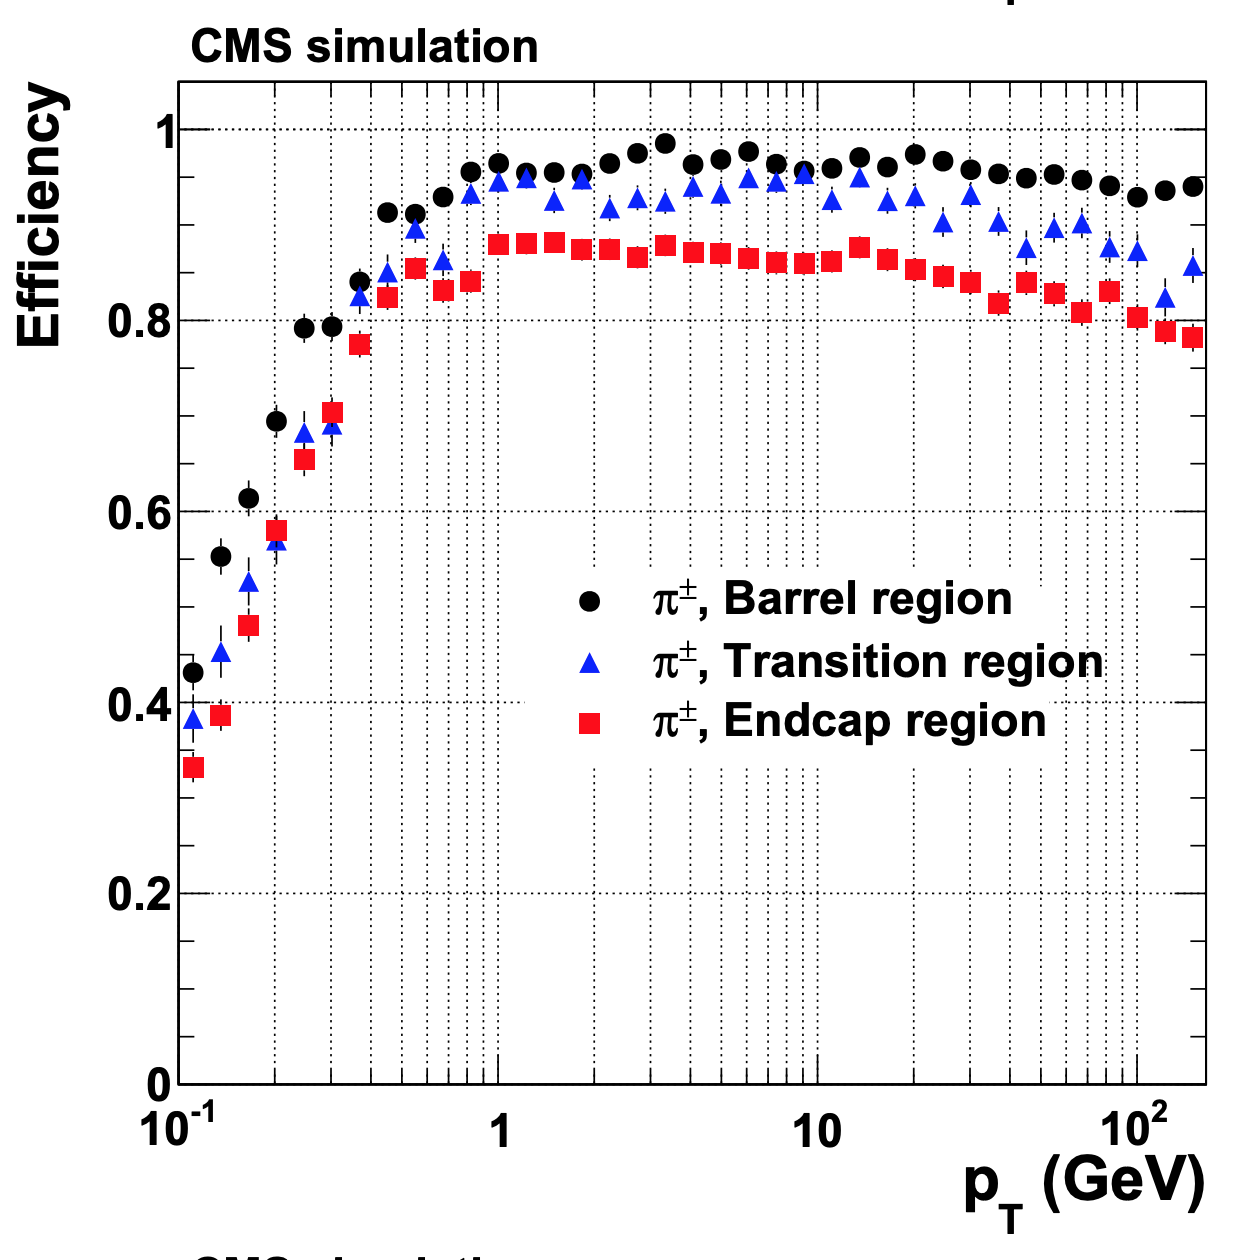
\includegraphics[width=0.31\linewidth]{figures/cms/cms_tracker_pion.png} &
        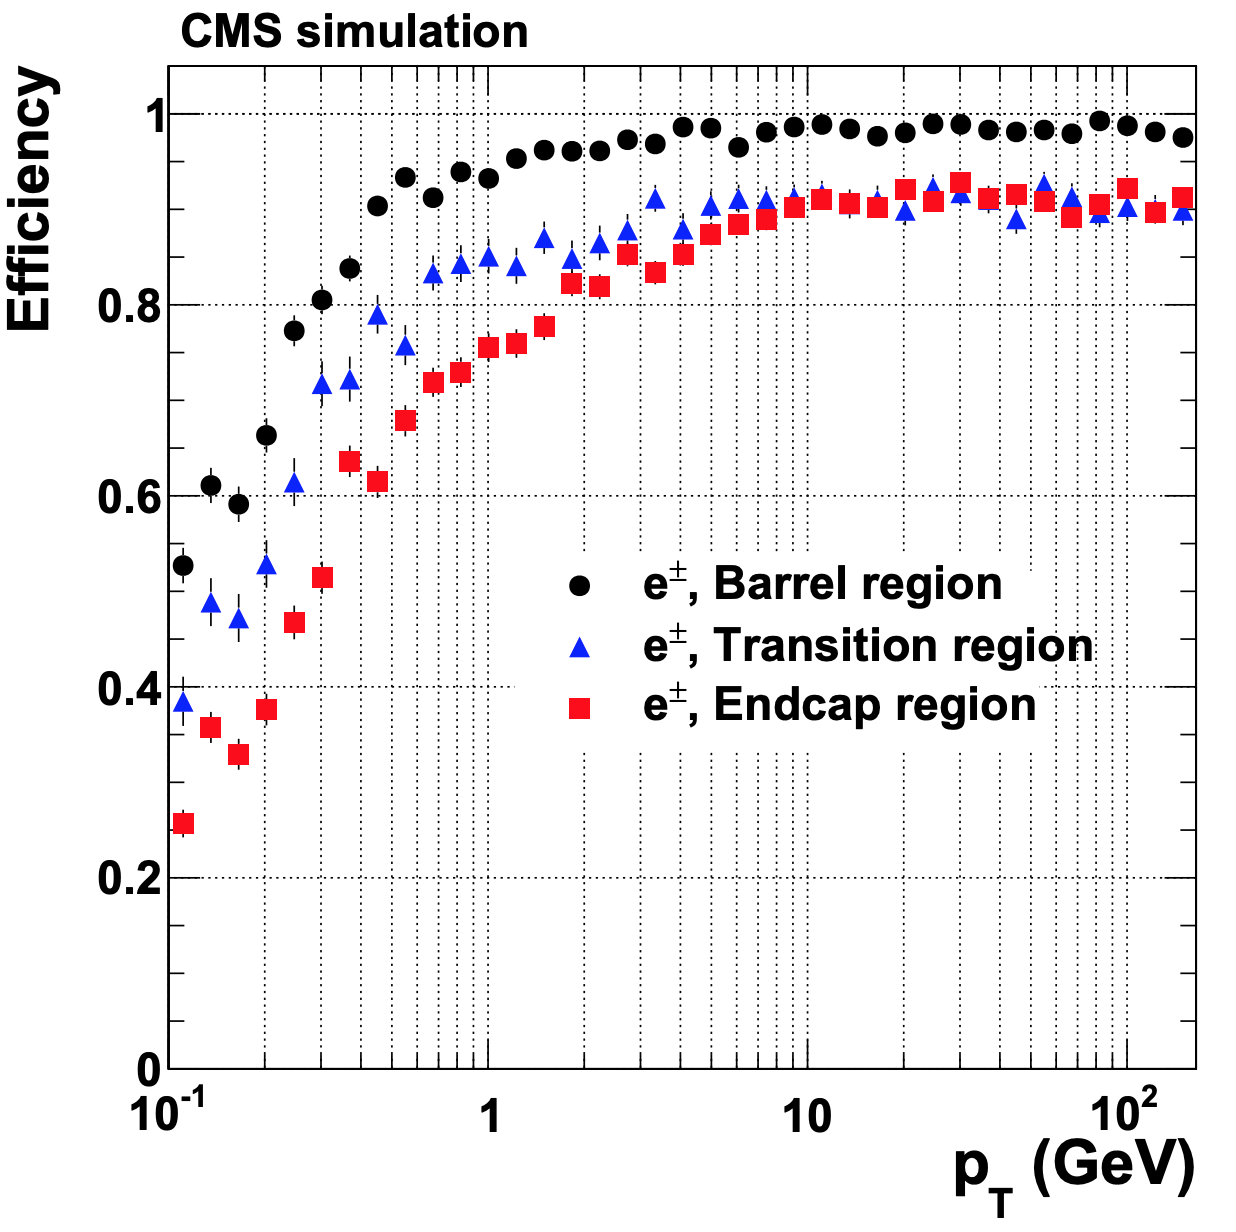
\includegraphics[width=0.31\linewidth]{figures/cms/cms_tracker_electron.png}
    \end{tabular}
    \caption{Tracking efficiency as a function of \pT for muons (left), charged pions (middle), and electrons (right), shown separately for the barrel (black), transition region (blue), and endcap (red). Taken from~\cite{Chatrchyan:1704291}.}
    \label{fig:cms_tracker_eff}
\end{figure}


\subsection{Electromagnetic Calorimeter} \label{sec:cms_ecal}
The primary goal of the CMS electromagnetic calorimeter is to preicsely measure the momenta of photons, especially important for studying the properties of the Higgs boson in the \Hgg channel.
Along with the tracker, the ECAL also assists in measurements of electrons which radiate a significant fraction of their energy through via bremsstrahlung as they pass through the detector.
Other charged particles, like charged pions and muons, interact relatively negligibly with the ECAL, as they emit a much smaller fraction of their energy via bremsstrahlung (due to the fact that they are much more massive than electrons).

The CMS ECAL is composed of over $6 \times 10^4$ lead tungstate (PbWO$_4$) crystals in the barrel and over $7 \times 10^3$ crystals in each of the endcaps, with the barrel component (EB) providing coverage up to $|\eta| \leq 1.479$ and the endcap components providing coverage from $1.479 \leq |\eta| \leq 3.0$~\cite{Chatrchyan:2008aa}.

Lead tungstate is an attractive choice for the ECAL crystals for several reasons, including its high density (8.28~g/cm$^3$), short radiation length (0.89~cm), and small Moliere radius (2.2~cm), defined as the average size of a cylinder containing 90\% of an incident photon or electron's energy.
The short radiation length allows the CMS ECAL to be compact, and the small Moliere radius allows for better spatial resolution of incident photons and electrons.
The former is important from a practical and financial point of view, as the ECAL must be placed within the HCAL and solenoid, while the latter is important as better spatial resolution allows for better diphoton and dielectron invariant mass resolution (assisting with idenitfying \Hgg and \Zee events).

Two additional attractive properties of lead tungstate include its short scintillation time and resistance to radiation damage.
The scintillation time must be on the order of the bunch crossing time at the LHC (25~ns) so that ECAL deposits from consecutive crossings can be distinguished from each other (a short bunch crossing time is desirable as it results in increased integrated luminosity).
Indeed, about 80\% of light is emitted within 25~ns within the CMS ECAL~\cite{Bayatian:2006nff}, allowing for high temporal resolution in the high luminosity conditions of the LHC.
Due to the high particle flux, radiation damage to detector components is inevitable; this results in wavelength-dependent loss of light transmission~\cite{Bayatian:2006nff}.
Although lead tungstate is particularly radiation-hard, the damage must still be tracked and corrected for by injecting laser light and monitoring the transparency of crystals.

Further details of the reconstruction of photons are described in Sec.~\ref{sec:evt_photon}.

\subsection{Hadronic Calorimeter} \label{sec:cms_hcal}
The CMS Hadronic Calorimeter (HCAL) is particularly important for measuring the momenta of neutral hadrons, the only detector subcomponent which is able to do so.
It also assists in the momenta measurements of charged hadrons, though the tracker is typically much more effective for this purpose.
Precisely measuring the momenta of hadrons allows for good energy resolution of hadronic jets -- this is important for constructing a reliable estimate of the missing transverse momentum in a given event.
Conversely, poor resolution of jet energies would result in poor resolution of the missing transverse momentum, degrading the experiment's ability to identify events in which there is true missing transverse momentum, either from neutrinos or yet-to-be discovered particles which do not interact with the CMS detector.
The CMS detector is typically able to achieve a mometum resolution of around 10\%~\cite{Bayatian:2006nff} for hadronic jets, using a combination of information from the various detector subcomponents.

The CMS HCAL is composed of two primary components: barrel (HB), covering $|\eta| \leq 1.4$ and endcap (HE), covering $1.3 \leq |\eta| \leq 3.0$.
The barrel component also contains a ``tail catcher'' placed outside the solenoid (HO), which covers up to $|\eta| \leq 1.26$.
Finally, a forward calorimeter (HF) specializes in measuring very forward particles, up to $|\eta| \leq 5$~\cite{Bayatian:2006nff}.
The various components of the HCAL and their pseudorapidity coverage are depicted in Fig.~\ref{fig:cms_hcal_schematic}.

\begin{figure} [htbp!]
    \centering
    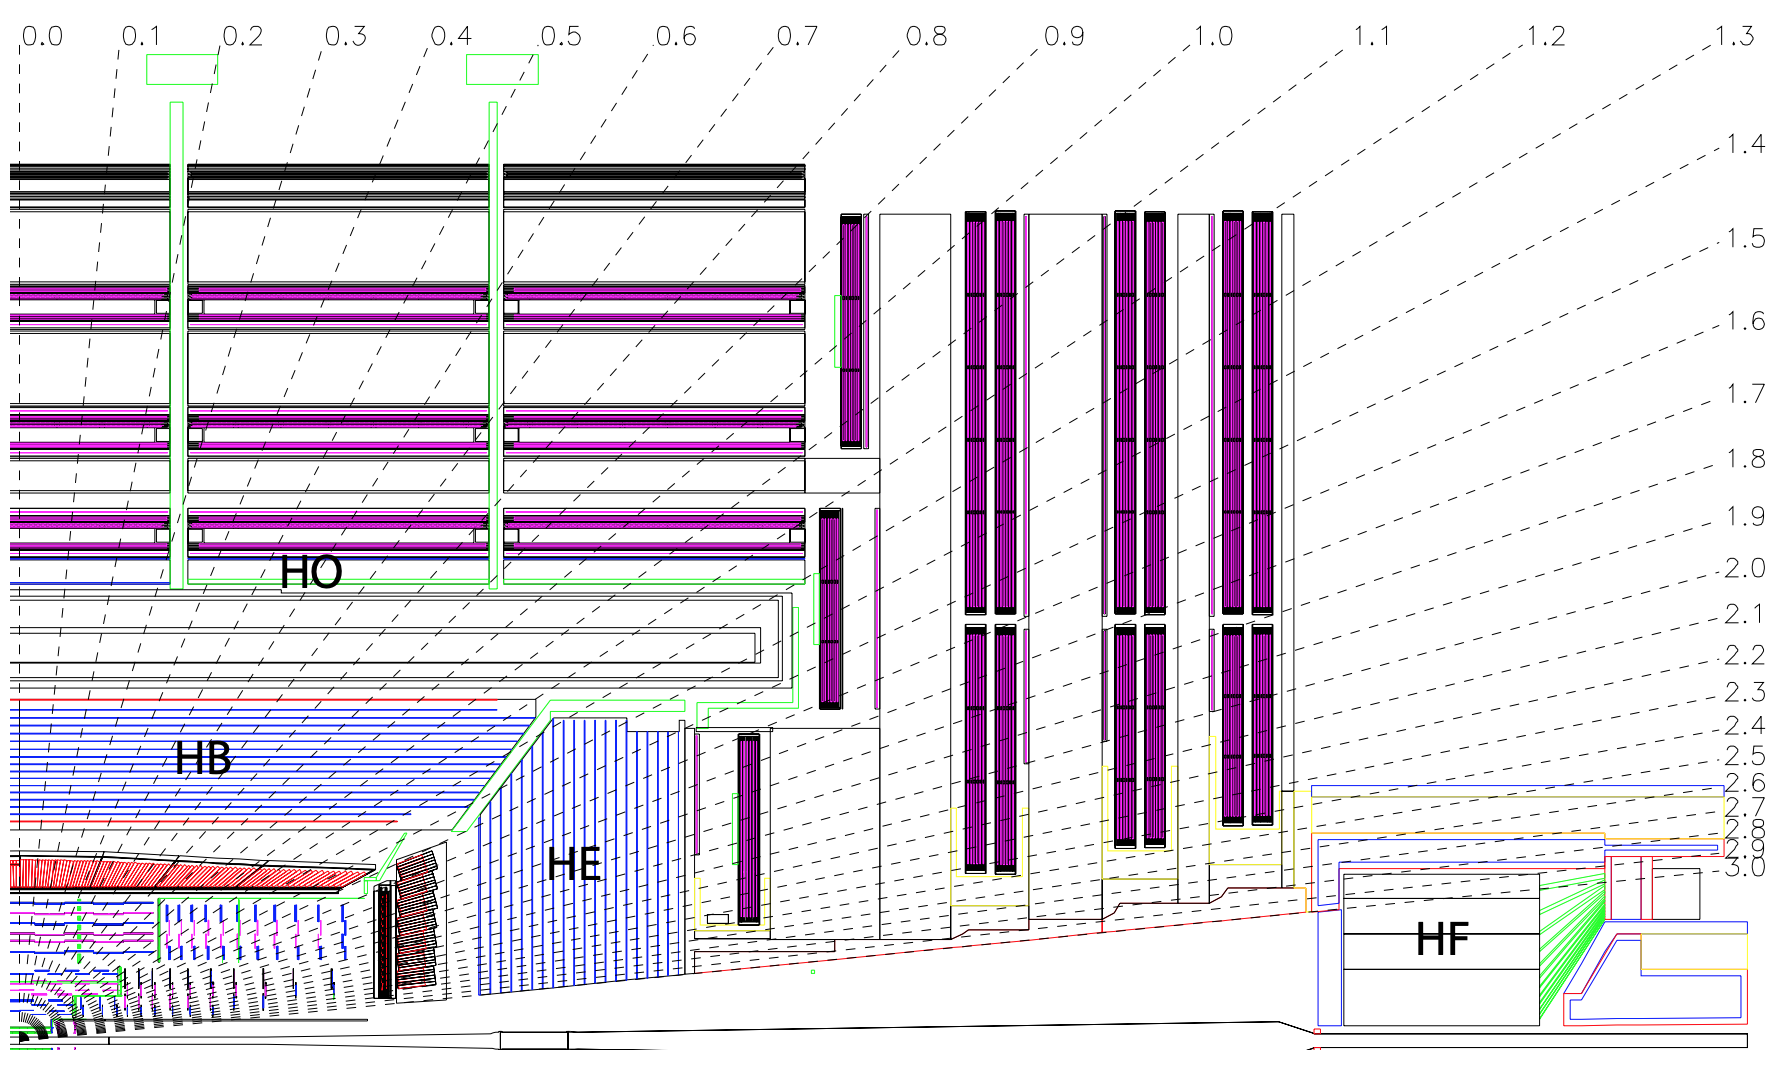
\includegraphics[width=0.7\linewidth]{figures/cms/hcal_schematic.png}
    \caption{Schematic of subcomponents of the CMS HCAL, along with their pseudorapidity coverage. Taken from~\cite{Chatrchyan:2008aa}.}
    \label{fig:cms_hcal_schematic}
\end{figure}

Conceptually, the HCAL aims to measure hadron energies by placing a high density of atomic nuclei, with which hadrons are likely to undergo nuclear (i.e. strong) interactions.
The products of these nuclear interactions are then measured with plastic scintillators and the HCAL is then able to reconstruct the energy of the original hadron.

In practice, this is achieved through brass alloy absorber plates with plastic scintillators interspersed between them~\cite{Bayatian:2006nff}.
To decrease the probability that hadrons ``punch through''~\cite{Belotelov:933703} the HCAL and leave the detector unmeasured, multiple layers of brass and plastic scintillators are utilized, with 17 layers total.

\subsection{Muon System} \label{sec:cms_muon_system}
The outermost detector subcomponent of the CMS detector is the muon system, placed outside the solenoid.
The primary goals of the muon system are to identify the presence of muons, measure their momenta, and provide the ability to trigger on events with muons~\cite{Chatrchyan:2008aa}.
Installing a second tracker outside the solenoid would be ideal, but in practice, this would be far too expensive.
A more economical solution is a detector using gas-filled chambers, exploiting the fact that muons traversing through the gas will ionize it.

The muon system is made of three components:
\begin{enumerate} 
    \item Drift tube (DT) chambers, which cover the region $|\eta| \leq 1.2$.
    \item Cathode strip chambers (CSC), which cover the region $0.9 \leq |\eta| \leq 2.4$.
    \item Resitive plate chamber (RPC) system, which is installed in both the barrel and endcap regions, covering $|\eta| \leq 1.6$.
\end{enumerate}

The DT chambers are well-suited to the barrel, where the muon rate and background rate are lower, while the CSCs, having better radiation resistance~\cite{Chatrchyan:2008aa}, are better suited to the endcaps, where the muon rate and background rate are higher.
The RPCs specialize in providing the ability to trigger on events with muons: although their position resolution is coarser than that of the DT chambers or CSCs, they provide excellent time resolution, allowing consecutive bunch crossings to be distinguished from one another.

The muon system is especially helpful in assisting in the measurement of high $p_{\text{T}}$ $\mathcal O$(TeV) muons.
As charged particles' energies are primarily determined through the curvature of their tracks, this presents a challenge for especially high energy particles: higher energy particles curve less and there is greater uncertainty on their respective momentum measurements.
Fig.~\ref{fig:cms_muon_vs_tracker} shows the momentum resolution for muons as a function of $p_{\text{T}}$.
While both the tracker and muon system are capable of measuring the momenta of muons of a wide range of energies, the muon system provides the greatest improvement to the overall resolution at very high $p_{\text{T}}$.

Beyond just improving the momentum resolution of high energy muons, the muon system is useful in the measurement of lower energy muons as well.
As the muon system and the tracker provide independent measurements of muons, this allows for fault-finding and cross-checks of each detector component.

\begin{figure} [htbp!]
    \centering
    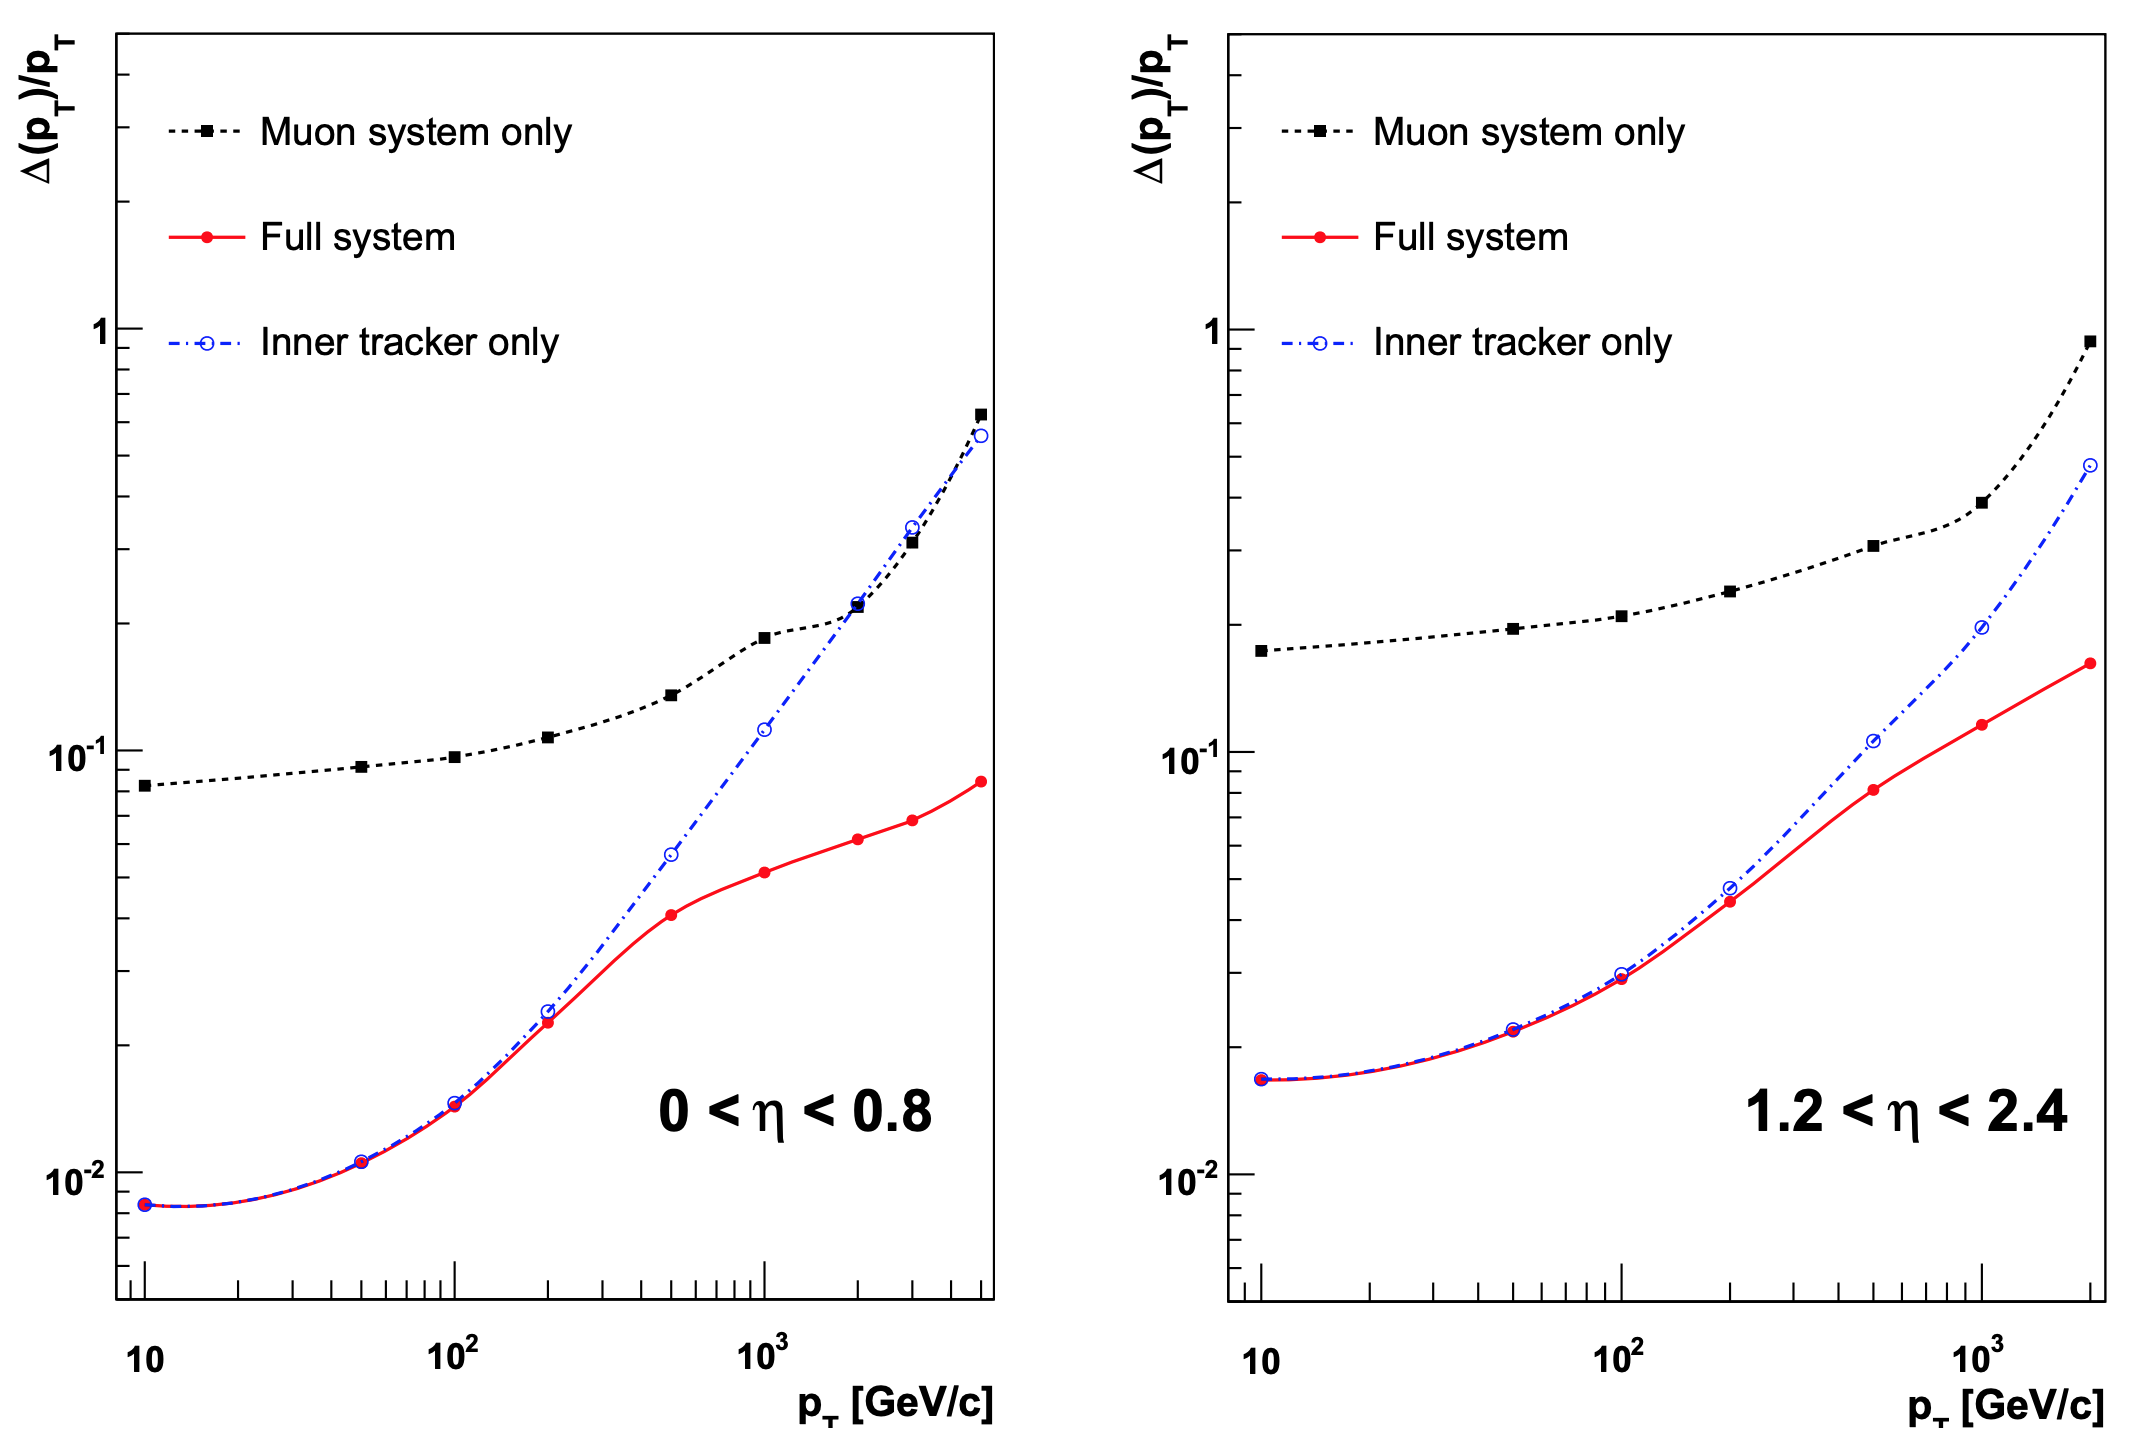
\includegraphics[width=0.8\linewidth]{figures/cms/cms_tracker_vs_muon.png}
    \caption{Fractional momentum resolution for muons reconstructed by the CMS detector, shown for reconstructions using the inner tracker only (blue), the muon system only (black), and the combination of measurements from both subdetectors (red). The muon system improves significantly the momentum resolution of $\mathcal O$(TeV) muons. Taken from~\cite{Chatrchyan:2008aa}.}
    \label{fig:cms_muon_vs_tracker}
\end{figure}

\subsection{Trigger System} \label{sec:cms_trigger}
At the LHC's design luminosity of $10^{34}$~cm$^{-2}$~s$^{-1}$, the pp interaction rate is greater than 1~GHz~\cite{Khachatryan:2016bia}.
It is neither necessary nor feasible to store the data of each of the more than $10^9$ events per second, as the vast majority of pp interactions are neither interesting nor useful in light of the goals of the CMS physics program.
It is not feasible in the sense that the CMS readout electronics impose an upper limit on the event rate of about 100~kHz, such that the vast majority of events must be thrown away.
Is is not necessary in the sense that most physics processes of interest have cross sections many orders of magnitude smaller than the nominal pp interaction cross section.

In order to select only the most interesting events to store for later analysis, a two-tiered trigger system is employed by the CMS detector.
The first level (L1), is implemented on custom hardware, and reduces the event rate by a factor of about $10^4$, from around 1~GHz to around 100~kHz.
The second level (HLT), is implemented in software, and further reduces the event rate to a typical rate of 400~Hz.

\subsubsection{L1 Trigger}
The L1 trigger combines information from the ECAL, HCAL, and muon system to decide with a fixed latency of 4~$\mu$s of a collision if the event should be accepted or not.
A schematic overview of the trigger system is shown in Fig.~\ref{fig:cms_l1_trigger}.
Events which pass the L1 trigger are then evaluated by the high-level trigger system to make a final decision on if the full event data will be stored.

\begin{figure} [htbp!]
    \centering
    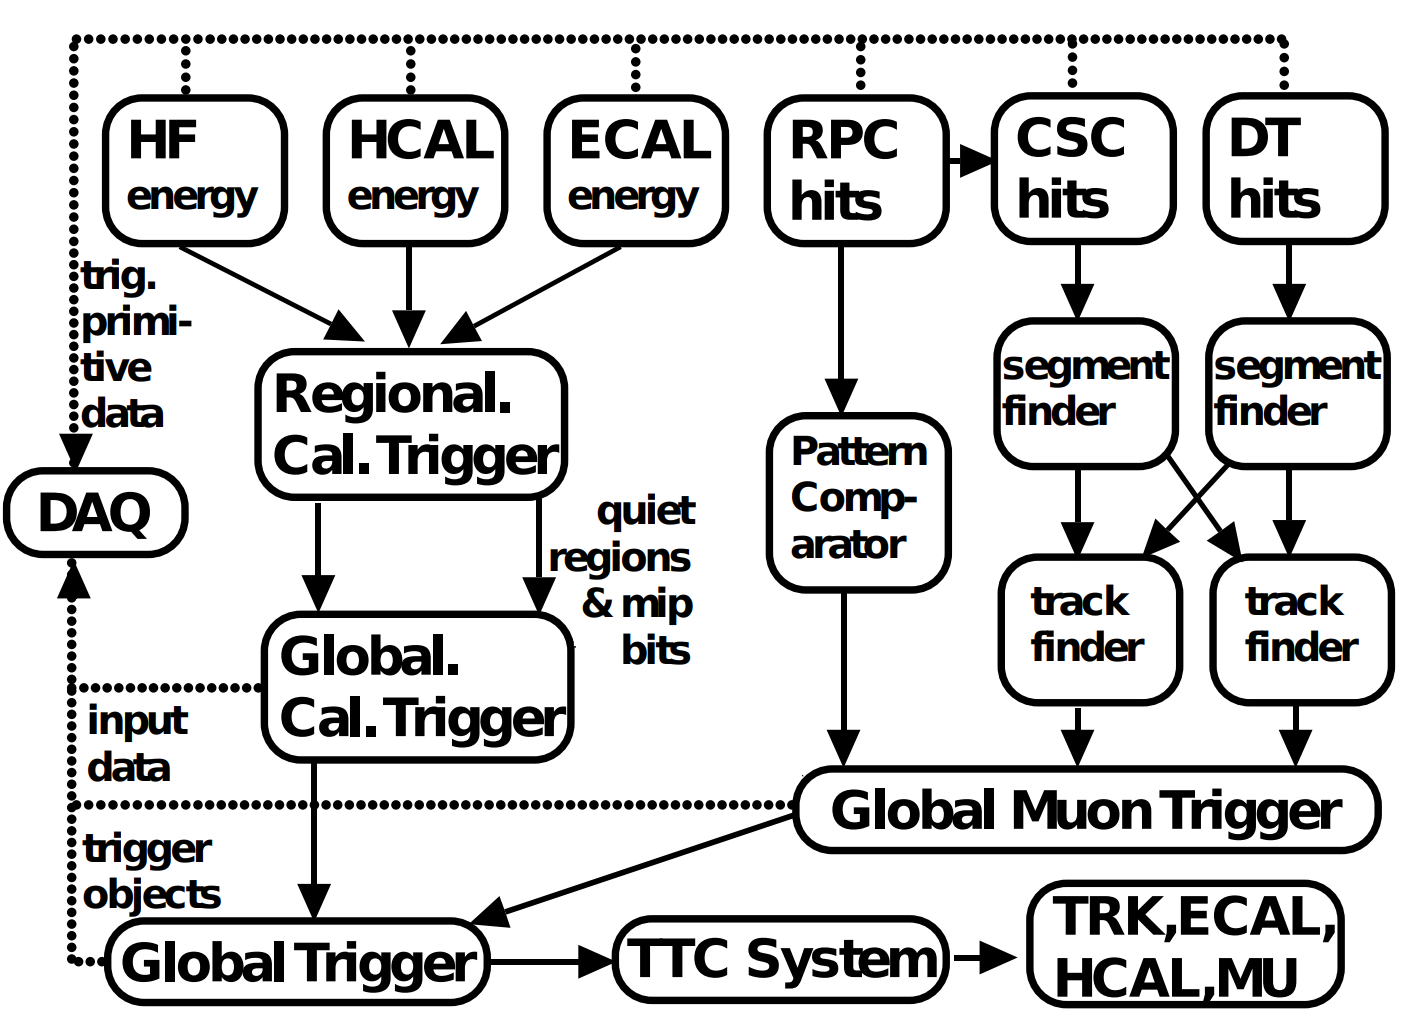
\includegraphics[width=0.6\linewidth]{figures/cms/cms_l1_trigger.png}
    \caption[Schematic overview of the CMS L1 trigger system. Taken from~\cite{Khachatryan:2016bia}.]{Schematic overview of the CMS L1 trigger system. Information from the calorimeters are first processed regionally and then a global calorimeter decision (GCT) is made. Similarly, information from the various components of the muon system are first processed regionally and then at a global level (GMT). The information from the global calorimeter trigger and global muon trigger are combined in a single global trigger (GT) which performs the final decision on whether to store the event. Taken from~\cite{Khachatryan:2016bia}.}
    \label{fig:cms_l1_trigger}
\end{figure}

\subsubsection{High-Level Trigger}
In contrast to the L1 trigger, the high-level trigger (HLT) system accepts events for storage based off a more complete, nearly offline-quality reconstruction of the event.
Details of event reconstruction, e.g. the particle flow algorithm, are describe in Sec.~\ref{sec:evt_pf}.
Near offline-quality event reconstruction is achieved in practice through the use of a ``processor farm'', a system of over $10^4$ CPUs working in parallel to efficiently reconstruct each event.
The HLT takes significantly longer to ``think'' about each event, with an average processing time on the order of 100~ms per event (compare to 4~$\mu$s for L1).

The high-level trigger paths used for the \ttH (\Hgg) analysis are the following:
\begin{itemize}
    \item 2016: \texttt{HLT\_Diphoton30\_18\_R9Id\_OR\_IsoCaloId\_AND\_HE\_R9Id\_Mass90*}
    \item 2017: \texttt{HLT\_Diphoton30\_22\_R9Id\_OR\_IsoCaloId\_AND\_HE\_R9Id\_Mass90*}
    \item 2018: \texttt{HLT\_Diphoton30\_22\_R9Id\_OR\_IsoCaloId\_AND\_HE\_R9Id\_Mass90*}
\end{itemize}

Conceptually, each of these triggers requires the presence of two photons with leading (subleading) transverse momenta of 30 (18/22) GeV, imposes requirements on the photons' shower shape variables (described in further detail in Sec.~\ref{sec:evt_photon}), and requires a diphoton invariant mass of at least 90 GeV.
The photon selection requirements described in Sec.~\ref{sec:evt_photon} are defined to be similar (and slightly stricter) than those of the trigger paths listed here.
Still, the efficiency of the trigger in simulation does not necessarily match that in data.
The efficiency is measured in data with \Zee events and the efficiency in simulation is accordingly corrected as a function of the transverse energy, pseudorapditity, and shower shape variable $R_9$ (defined in Sec.~\ref{sec:evt_photon}), with the uncertainty on the scale factor taken as a systematic uncertainty (described in Sec.~\ref{sec:tth_systematic_uncertainties}). 

